\documentclass{article}
\usepackage{graphicx} 
\usepackage{tikz}
\usetikzlibrary{positioning, arrows.meta}
\usepackage{caption}
\usepackage[T1]{fontenc}
\usepackage{xcolor}          
\usepackage{listings} 
\usepackage{amsmath}
\usepackage{booktabs} 
\usetikzlibrary{matrix}
\usepackage{float}
\usepackage{subcaption}
\usetikzlibrary{plotmarks}          
\usepackage{pgfplots}                 
\pgfplotsset{compat=1.18}            
\usepgfplotslibrary{groupplots}  
% \usepackage[
%   left=2.5cm,
%   right=2.5cm,
%   top=2.0cm,
%   bottom=2.0cm
% ]{geometry}
\usepackage[
    backend=biber,   
    style=numeric,      
    sorting=none         
]{biblatex}
\usepackage{hyperref}
\hypersetup{
    colorlinks=false,
    pdfborder={0 0 0}
}

\lstdefinestyle{cppclean}{
  language        = C++,    
  basicstyle      = \ttfamily\small,  
  keywordstyle    = \color{blue}\bfseries,
  commentstyle    = \color{green!50!black}\itshape,
  stringstyle     = \color{red!70!black},
  numberstyle     = \tiny\color{gray},
  numbers         = left,     
  stepnumber      = 1,
  numbersep       = 10pt,
  backgroundcolor = \color{gray!05}, 
  frame           = single,
  rulecolor       = \color{gray!50},
  columns         = flexible,
  tabsize         = 4,
  showstringspaces= false,
  captionpos      = b, 
  breaklines      = true,
  breakatwhitespace = true
}
\lstset{style=cppclean}
\addbibresource{references.bib}

\definecolor{hwloc-color-255-255-255}{RGB}{255,255,255}
\definecolor{hwloc-color-0-0-0}{RGB}{0,0,0}
\definecolor{hwloc-color-255-255-255}{RGB}{255,255,255}
\definecolor{hwloc-color-255-255-255}{RGB}{255,255,255}
\definecolor{hwloc-color-210-231-164}{RGB}{210,231,164}
\definecolor{hwloc-color-231-255-181}{RGB}{231,255,181}
\definecolor{hwloc-color-231-255-181}{RGB}{231,255,181}
\definecolor{hwloc-color-190-190-190}{RGB}{190,190,190}
\definecolor{hwloc-color-255-255-255}{RGB}{255,255,255}
\definecolor{hwloc-color-239-223-222}{RGB}{239,223,222}
\definecolor{hwloc-color-242-232-232}{RGB}{242,232,232}
\definecolor{hwloc-color-255-255-255}{RGB}{255,255,255}
\definecolor{hwloc-color-190-210-149}{RGB}{190,210,149}
\definecolor{hwloc-color-222-222-222}{RGB}{222,222,222}
\definecolor{hwloc-color-255-255-255}{RGB}{255,255,255}
\definecolor{hwloc-color-255-255-255}{RGB}{255,255,255}
\definecolor{hwloc-color-0-255-0}{RGB}{0,255,0}
\definecolor{hwloc-color-255-0-0}{RGB}{255,0,0}
\definecolor{hwloc-color-255-255-0}{RGB}{255,255,0}


\title{Cache-Oblivious: VanEmde-Boas-Trees}
\author{Jakob Eberhardt \\ \texttt{jakob.eberhardt@estudiantat.upc.edu}}
\date{\today}

\begin{document}

\maketitle
\thispagestyle{empty}
\newpage
\setcounter{page}{1}
\tableofcontents
\lstlistoflistings
\listoffigures
\listoftables
\newpage 


\section{Introduction \& Problem Statement}
\label{sec:intro}
In this assignment, we will employ VanEmde-Boas-Trees to study the benefits and importance of cache-optimized programming. Many workloads, e.g. database or graphics applications are so-called \textit{memory bound}, meaning that their overall performance is dictated by how fast the CPU can read and write data to compute the problem. Although nowadays DRAM memory is typically available at a sufficiently low price, the latency for bringing data from DRAM or other external memories into the CPU is too long to saturate the CPU's capabilities in terms of computation, because the pipeline of a core in the CPU has to stall while waiting for data from a slow memory. To address this, microarchitects added multiple levels of increasingly fast but hence also more expensive memories in between the CPU and the external memories. These so-called caches are organized in lines of memory and enable the programmer to exploit temporal and spatial locality, meaning that the faster cache memory will hold the values of recently used variables and those that are close to it and likely accessed in the future. However, faster cache memories are expensive and hence many orders of magnitude smaller than the main memory, as can be seen in table~\ref{tab:mem}. Therefore, if the CPU requests data while the respective cache level is already filled up, a cache line has to be evicted according to a certain policy, e.g. the least recently used line. 

\begin{table}[h]
  \centering
  \caption[Memory Hierarchy]{Typical 2025 desktop memory hierarchy~\cite{lam2025}~\cite{crucialDDR5}~\cite{olmez2024}. Caches are further decided in lines that can hold more than one variable of a program. The typical size is 64 bytes.}
  \begin{tabular}{lcc}
    \toprule
    \textbf{Memory level} & \textbf{Typical capacity} & \textbf{Typical latency} \\
    \midrule
    Registers         & $\sim$2\,\text{KB}   & $\sim$0.3\,ns \\
    L1 Cache              & $\sim$192\,\text{KB} & $\sim$0.6\,ns \\
    L2 Cache              & $\sim$3\,\text{MB}   & $\sim$2\,ns   \\
    L3 Cache              & $\sim$36\,\text{MB}  & $\sim$12\,ns  \\
    Main Memory (DDR5)    & $\sim$32\,\text{GB}  & $\sim$90\,ns  \\
    Hard-Disk Drive       & $\sim$8\,\text{TB}   & $\sim$5\,ms   \\
    \bottomrule
  \end{tabular}
\end{table}
\label{tab:mem}

Since the cache resources are scarce, it requires the programmer to minimize the amount of expected cache misses in order to achieve higher levels of performance. In this case, we are considering binary search trees which we will construct and then query. To keep the experiment concise, we will only consider searches and will not mutate the tree after the initialization. We will compare the implementation of a plain search tree and a recursively built VanEmde-Boas tree in terms of their memory footprint and impact on caching. 

\section{Interface}
In listing~\ref{lst:interface}, we see the abstract interface for our BST implementations. We support three operations which are \texttt{insert} which allows us to insert an arbitrary \texttt{Key} into the tree, e.g. a \texttt{std::int64\_t} integer value which we will use throughout the benchmarks. We will look up these keys using the \texttt{contains} function which will return true or false. Lastly, we define a \texttt{size\_bytes()} function which is a helper function to return the used memory for a given implementation. 

\begin{lstlisting}
template<class Key>
class IBST {
public:
    virtual void insert(const Key& k)                = 0;
    virtual bool contains(const Key& k)        const = 0;
    virtual std::size_t size_bytes()           const = 0;
    virtual ~IBST() = default;
};
\end{lstlisting}
\captionof{lstlisting}[Abstract Interface for BSTs in \texttt{IBST.h}]{Abstract interface class for our Binary Search Tree implementation in \texttt{IBST.h}}
\label{lst:interface}
The interface class will help us to avoid code duplication and also facilitate the creation of benchmarking instances. In the following sections~\ref{sec:plain} \&~\ref{sec:vb} we will break down the actual implementations. The full code can be seen in the appendix section~\ref{sec:app}

\section{Plain Binary Search Tree Implementation}
\label{sec:plain}
In this section, we will break down the plain and canonical pointer binary search trees and their respective effects on memory layout. As can be seen in listing~\ref{lst:btrfields}, the \texttt{BSTPtr} class implements our interface. To this end, we have to keep three data fields wrapped into the \texttt{Node} struct: 
\begin{enumerate}
    \item \texttt{Key}: E.g. a \texttt{std::int64\_t} integer with eight bytes
    \item \texttt{l}~\&~\texttt{r}: Two \texttt{std::unique\_ptr} pointers pointing to the left and right child node, each eight bytes. 
\end{enumerate}
Although the total memory used for the struct is 24 bytes, we probably have to take machine-specific padding and allocation memory overheads into account. 
\begin{lstlisting}
template<class Key>
class BSTPtr : public IBST<Key> {
    struct Node {
        Key key;
        std::unique_ptr<Node> l, r;
        explicit Node(const Key& k) : key(k) {}
    };

    std::unique_ptr<Node> root_;
    std::size_t node_cnt_ = 0;
};
\end{lstlisting}
\captionof{lstlisting}[\texttt{BSTPtr} Class \& Data Fields in \texttt{BSTPtr.h}]{Plain Binary Search Tree implementation in \texttt{BSTPtr.h}}
\label{lst:btrfields}
Additionally, we keep the root of our tree in \texttt{root\_}. Hence, it will always be referenced when we later start to traverse the tree. Lastly, we keep the \texttt{node\_cnt\_} variable to later implement the \texttt{size\_bytes()} function. This can be seen in listing~\ref{lst:bstins} where we increment it every time we insert a node. The used memory can simply be computed by $node\_cnt\_ \times sizeof(Node)$.

\subsection{Why Plain Insertion may be a Problem}
The insertion of nodes into the tree is the critical point when looking at cache optimizations. In listing~\ref{lst:bstins}, we see how new nodes are inserted. 
\begin{lstlisting}
void insertNode(std::unique_ptr<Node>& p, const Key& k) {
        if (!p) {
            p = std::make_unique<Node>(k);
            ++node_cnt_;                         
        } else if (k < p->key) {
            insertNode(p->l, k);
        } else if (k > p->key) {
            insertNode(p->r, k);
        }
    }
\end{lstlisting}
\captionof{lstlisting}[Plain Node Insertion in \texttt{BSTPtr.h}]{The internal \texttt{insertNode} implementation for standard BST in \texttt{BSTPtr.h}}
\label{lst:bstins}
We use \texttt{std::make\_unique<Node>(k)} to allocate a new \texttt{Node} when the call to \texttt{insertNode} reaches a null pointer in order to obtain a unique pointer. If we check the C++-specific implementation in \texttt{unique\_pointer.h} seen in listing~\ref{lst:internals}, we see that this allocation happens on the heap, since the \texttt{new} keyword is used. Since the allocator will try to minimize the fragmentation on the heap, it likely will fill gaps in the heap with the small \texttt{Node} objects. This may cause performance issues since the memory addresses of two nodes which were created one after another may not map to the same cache line. During an insertion the algorithm walks from the root to the future parent of the new node, performing one key comparison per level.  At each step, it dereferences either \texttt{l} or \texttt{r}, e.g. a pointer that almost certainly points to a line that is not yet in the cache.  Hence, a random-order build of an $n$-node tree incurs $\Theta(n \log n)$ cache misses in addition to the usual $\Theta(n \log n)$ comparisons which is often the defining runtime factor.



\begin{lstlisting}
template<typename _Tp, typename... _Args>
    _GLIBCXX23_CONSTEXPR
    inline __detail::__unique_ptr_t<_Tp>
    make_unique(_Args&&... __args)
    { return unique_ptr<_Tp>(new _Tp(std::forward<_Args>(__args)...)); }
\end{lstlisting}
\captionof{lstlisting}[Heap Allocation in \texttt{unique\_pointer.h}]{The implementation of \texttt{std::make\_unique<Node>(k)} in \texttt{unique\_pointer.h} calling \texttt{new} for each node.}
\label{lst:internals}

We will experimentally investigate if and how this allocation pattern which happens at construction time will affect the performance and cache-friendliness of the \texttt{contains} function of our plain BST. As can be seen in listing~\ref{lst:containsbst}, we will start at the root node and iteratively decent the tree until we either find the key or encounter a null pointer. Hence, for every level we perform at most one comparison and one pointer dereference which may cause a cache miss. 
\begin{lstlisting}
static bool contains(const std::unique_ptr<Node>& p, const Key& k) {
        const Node* cur = p.get();
        while (cur) {
            if (k == cur->key) return true;
            cur = (k < cur->key) ? cur->l.get() : cur->r.get();
        }
        return false;
    }
\end{lstlisting}
\captionof{lstlisting}[The \texttt{contains} implementation of Plain BSTs in \texttt{BSTPtr.h}]{The \texttt{contains} implementation of Plain BSTs in \texttt{BSTPtr.h}}
\label{lst:containsbst}

\subsection{Example}
\label{secsec:explain}
Even without fragmentation, there are reasons why a more sophisticated layout may be useful. In this example, we represent the integer keys 1-7 in memory according to the previously described plain binary search tree implementation, ensuring it remains perfectly balanced. During the experimentation, we used a random input order. In this case, we use a defined sequence in order to make the example comparable to the VEB implementation. The example tree can be seen in figure~\ref{fig:extree}. If we apply the node insertion according to the code in listing~\ref{lst:bstins}, we see in figure~\ref{fig:plainmem} that although the subtree 4-2-6 will likely be located closely in memory, the subtree of 6, however, is separated from its children nodes which hence may map to different cache lines. 
\input{tree}
\begin{figure}[h]
  \centering
  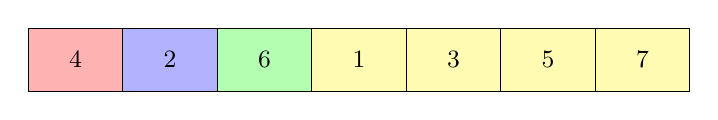
\begin{tikzpicture}
    \def\w{1.2} 
    \def\h{0.8}   

    \foreach \key/\col [count=\i from 0] in {4/red!30, 2/blue!30, 6/green!30,
                                             1/yellow!30, 3/yellow!30,
                                             5/yellow!30, 7/yellow!30}{
      \draw[fill=\col] (\i*\w,0) rectangle ++(\w,\h);
      \node at (\i*\w+0.5*\w,0.5*\h) {\small \key};
    }
  \end{tikzpicture}
  \caption[Plain BST Insertion Example]{Plain BST insertion (level-order) memory blocks.}
  \label{fig:plainmem}
\end{figure}



\section{Van Emde-Boas Tree Implementation}
\label{sec:vb}
Next, we will present the implementation of the Van Emde-Boas strategy for trees. The full implementation can be seen in the appendix section~\ref{secsec:vb}. First, if we consider the data fields of this implementation seen in listing~\ref{ls:datavb}, we see that we keep two vectors of our selected keys. We have to acknowledge that we do not rely on pointers to organize the data. We will see later how simple arithmetic will still allow us to query the tree efficiently with a smaller memory footprint.  The array \texttt{inserts\_} is an intermediate buffer for sorting out the insertion order of the keys. Once it is in the correct order, we will set the sentinel boolean variable \texttt{frozen\_} to true which marks the actual and now immutable VEB array \texttt{a\_} as valid.
\begin{lstlisting}
template<class Key>
class BSTVEB : public IBST<Key> {
    std::vector<Key> a_;            
    bool              frozen_ = false;
    std::vector<Key>  inserts_; 
\end{lstlisting}
\captionof{lstlisting}[Data Fields of the Van Emde-Boas Tree Implementation in \texttt{BSTVEB.h}]{Data Fields of the Van Emde-Boas Tree Implementation in \texttt{BSTVEB.h}}
\label{ls:datavb}

For a VEB tree, we aim at placing every complete subtree that is small enough to fit in one cache line stored contiguously in memory. To this end, we need a more sophisticated algorithm. Once we start to query the tree, we lock the insertion queue using the \texttt{freeze} function seen in listing~\ref{ls:freez}. We sort the \texttt{inserts\_} array and remove duplicates. Once the data is prepared, we paste the array to our \texttt{a\_} array and start to recursively build the layout, as can be seen in listing~\ref{ls:vebinsert}.
\begin{lstlisting}
void freeze() {
        if (frozen_) return;

        std::sort(inserts_.begin(), inserts_.end());
        inserts_.erase(std::unique(inserts_.begin(), inserts_.end()),
                       inserts_.end());

        a_.reserve(inserts_.size());
        help::build_veb(a_, inserts_, 0, inserts_.size());
        frozen_ = true;
    }
\end{lstlisting}
\captionof{lstlisting}[Freezing \& Processing for Van Emde-Boas Tree Insertion Implementation in \texttt{BSTVEB.h}]{Freezing \& Processing for Van Emde-Boas Tree Insertion Implementation in \texttt{BSTVEB.h}}
\label{ls:freez}

The helper function \texttt{build\_veb} will recursively generate the cache-oblivious layout. To this end, we find the median element of our input array and save it as the next index of our output array. Since the input is already ordered, in other words, we select the root of the current subtree and put it into the next memory address. Afterwards, we recursively build the layout for the left, then right subtree. 
\begin{lstlisting}
void build_veb(std::vector<Key>& out,
               const std::vector<Key>& sorted, std::size_t lo, std::size_t hi)
{
    if (lo >= hi) return;                       
    std::size_t mid = (lo + hi) / 2;            
    out.push_back(sorted[mid]);                 
    build_veb(out, sorted, lo, mid);            
    build_veb(out, sorted, mid + 1, hi);        
}
} 
\end{lstlisting}
\captionof{lstlisting}[Insertion for Van Emde-Boas Tree Implementation in \texttt{BSTVEB.h}]{Insertion for Van Emde-Boas Tree Implementation in \texttt{BSTVEB.h}}
\label{ls:vebinsert}

The \texttt{containsRec} function seen in listing~\ref{ls:vebcontains} performs a binary search over the VEB-ordered array \texttt{a\_}. The arguments \texttt{lo} and \texttt{hi} limit the sorted key range. The \texttt{idx} variable points to the root of that range. If the range is empty, we return false, meaning we did not find the key and there are no segments left to explore. Otherwise, we compare the search key with \texttt{a\_[idx]} and succeed immediately on a match. We then calculate the midpoint \texttt{mid} in the same way as during the construction phase of the layout. We observe that the left subtree occupies \texttt{left\_size} = \texttt{mid} - \texttt{lo} elements immediately after the root, so the left and right children live at \texttt{idx} + 1 and \texttt{idx} + 1 + \texttt{left\_size} respectively.
Because those child indices are obtained by simple arithmetic instead of stored pointers, the search remains pointer-free while correctly descending the tree until we find the key or not.
\begin{lstlisting}
bool containsRec(const Key& k,
                std::size_t lo, std::size_t hi, std::size_t idx) const
    {
    if (lo >= hi) return false;            

    const Key& key = a_[idx];
    if (k == key) return true;

    std::size_t mid        = (lo + hi) / 2;
    std::size_t left_size  = mid - lo;    
    std::size_t left_idx   = idx + 1;   
    std::size_t right_idx  = idx + 1 + left_size;

    return (k < key)
        ? containsRec(k, lo, mid,           left_idx)
        : containsRec(k, mid + 1, hi,       right_idx);
    }
\end{lstlisting}
\captionof{lstlisting}[Recursive \texttt{contains} Function for Van Emde-Boas Tree Implementation in \texttt{BSTVEB.h}]{Recursive \texttt{contains} Function for Van Emde-Boas Tree Implementation in \texttt{BSTVEB.h}}
\label{ls:vebcontains}

The live memory that will be required during query time for the VEB implementation is given by the \texttt{size\_bytes} function seen in listing~\ref{ls:vebmemde}. Since this implementation works pointer-free, we only need eight bytes to store an integer, unlike the plain implementation which requires 24. Hence, we can simply multiply the unique amount of keys we have by their size, e.g. eight for a \texttt{std::int64\_t} integer. 
\begin{lstlisting}
std::size_t size_bytes() const override { return a_.size() * sizeof(Key); }
\end{lstlisting}
\captionof{lstlisting}[Memory Size for Van Emde-Boas Tree Implementation in \texttt{BSTVEB.h}]{Cpmputing the required memory for the pointer-free Van Emde-Boas Tree implementation in \texttt{BSTVEB.h}}
\label{ls:vebmemde}


\subsection{Example}
In this example, we will lay out the same keys seen in section~\ref{secsec:explain}, but according to the Van Emde-Boas layout. The sequence can be seen in table~\ref{tab:vebtab}. After we sorted the keys 1-7, we picked the median element 4 to be the root of the tree since it evenly divides the segment. Hence, it will get the VEB-index 0 or respectively the first address in memory as can be seen in figure~\ref{fig:vebmem}. Afterwards, we repeat the same procedure for the left subtree 0-3 where 2 will become the root and VEB-index 1. Equally, we repeat the recursion on the left tree which now only contains 1, hence it becomes VEB-index 2 and we continue with the right subtree of its sibling which will also return and become VEB-index 3. 
\begin{table}[h!]
  \centering
  \caption[VEB Array Layout Table]{VEB layout for the 7-key example.}
  \label{tab:veb7}
  \begin{tabular}{cccc}
    \toprule
    \textbf{VEB idx} & \textbf{Key} & \textbf{Segment [lo,\,hi)} & \textbf{Reason} \\
    \midrule
    0 & 4 & {[0,7)} & root of entire tree \\
    1 & 2 & {[0,3)} & root of left half \\
    2 & 1 & {[0,1)} & leaf \\
    3 & 3 & {[2,3)} & leaf \\
    4 & 6 & {[4,7)} & root of right half \\
    5 & 5 & {[4,5)} & leaf \\
    6 & 7 & {[6,7)} & leaf \\
    \bottomrule
  \end{tabular}
\end{table}
\label{tab:vebtab}

\begin{figure}[h]
  \centering
  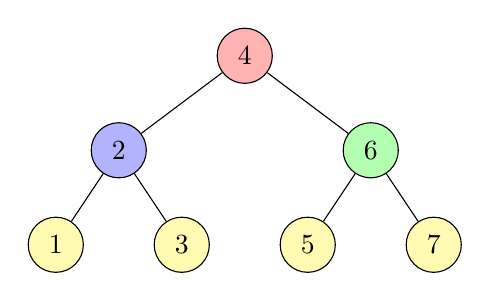
\begin{tikzpicture}[
      level distance = 12mm,
      every node/.style   = {circle, draw, minimum size=7mm, inner sep=0pt},
      level 1/.style      = {sibling distance=32mm},
      level 2/.style      = {sibling distance=16mm}
    ]
    \node[fill=red!30] {4}
      child { node[fill=blue!30] {2}
        child { node[fill=yellow!30] {1} }
        child { node[fill=yellow!30] {3} }
      }
      child { node[fill=green!30] {6}
        child { node[fill=yellow!30] {5} }
        child { node[fill=yellow!30] {7} }
      };
  \end{tikzpicture}
  \caption{Binary-search tree arranged in VEB array order.}
\end{figure}

After we resolve the whole recursive building phase, we can observe how the children of the subtree roots 2 and 6 are located sequentially after them in memory which increases the chances that they will be co-located in the same cache line. We will set up an experiment to check this theoretical guarantee in section~\ref{sec:ex}.
\begin{figure}[h]
  \centering
  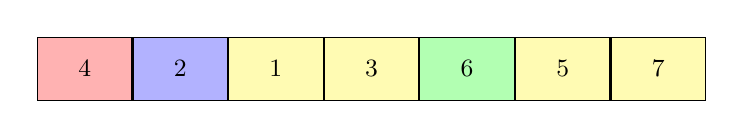
\begin{tikzpicture}
    \matrix[matrix of nodes,
            nodes={draw, minimum width=1.2cm, minimum height=8mm, font=\small},
            row sep=0pt, column sep=0pt] {
      |[fill=red!30]| 4 &
      |[fill=blue!30]| 2 &
      |[fill=yellow!30]| 1 &
      |[fill=yellow!30]| 3 &
      |[fill=green!30]| 6 &
      |[fill=yellow!30]| 5 &
      |[fill=yellow!30]| 7 \\
    };
  \end{tikzpicture}
  \caption[Memory View for the VEB-ordered Layout]{Memory View for the VEB-ordered layout}
  \label{fig:vebmem}
\end{figure}


\section{Experiment}
\label{sec:ex}
In this section, we will introduce the experimental setup which will be used to benchmark the previously described implementations.  An example of a configuration can be seen in listing~\ref{lst:exampleinstancels} below. The parameter \texttt{n} is the total amount of keys we will insert upon a benchmark. The number of lookups is defined in the \texttt{q} parameter and \texttt{T} is the number of experiment repetitions. The \texttt{csv} flag is for plotting output and \texttt{seed} specifies the random number generator seed.
\begin{lstlisting}
{
  "n"   : 100000,
  "q"   : 100000,
  "T"   : 5,
  "csv" : false,
  "seed": 123
}
\end{lstlisting}
\captionof{lstlisting}[Example Instance\texttt{small.json}]{A small example instance configuration in \texttt{data/small.json}}
\label{lst:exampleinstancels}


We will compare the implementations and instance results in terms of the following metrics. We compute the averages among the \texttt{T} experiment repetitions:
\begin{itemize}
    \item \textbf{Total Execution Time (\texttt{total\_ns})}: Average time (ns) taken to run a benchmark with a specific configuration (total time/\texttt{T})
    \item \textbf{Nanoseconds per Search (\texttt{ns/search})}: Average time (ns) taken for one lookup (\texttt{contains} function) (total query Time/\texttt{T})
    \item \textbf{Total L3 Cache References (\texttt{cache\_refs})}: Average total L3 cache references (total cache references/\texttt{T})
    \item \textbf{Total L3 Cache Misses (\texttt{cache\_misses})}: Average total L3 cache misses (total cache misses/\texttt{T})
    \item \textbf{Bytes in Use (\texttt{bytes(MB)})}: Bytes required to hold the \texttt{n} nodes
\end{itemize}


\subsection{Experiment Driver}
Listing~\ref{ls:exdriver} shows how we generate and process an experiment run. We can specify the variants we want to compile, e.g. the pointer-based BST implementation. By using a \texttt{Factory} pattern, we facilitate the integration of future implementations. For the insertion input, we generate \texttt{n} keys. Likewise, we populate a vector of length \texttt{q} with keys we will query during the benchmark. We accumulate the metrics over the \texttt{T} runs and compute their averages. 
\begin{lstlisting}
const std::vector<Variant> variants = {
    {"BST_PTR", [] { return std::make_unique<BSTPtr<int>>(); }},
    {"BST_VEB", [] { return std::make_unique<BSTVEB<int>>(); }},
};

void runExperiment(int n, int q, int T, bool csv,
                   const Factory& make, unsigned seed,
                   const std::string& impl)
{
    std::mt19937 rng(seed);
    std::uniform_int_distribution<int> dist(1, n * 10);

    std::vector<int> inserts(n);
    for (int& x : inserts) x = dist(rng);

    std::vector<int> lookups(q);
    for (int& x : lookups) x = dist(rng);

    long long  acc_ns   = 0;
    long long  acc_refs = 0, acc_miss = 0;
    std::size_t bytes_used = 0;

    for (int t = 0; t < T; ++t) {
        auto tree = make();
        Metrics m = benchOnce(*tree, lookups, inserts);
        acc_ns   += m.ns;
        acc_refs += m.cache_refs;
        acc_miss += m.cache_miss;
        if (t == 0) bytes_used = tree->size_bytes();  
    }

    double avg_ns      = double(acc_ns)   / T;
    double ns_per_op   = avg_ns / q;

    double avg_refs    = double(acc_refs) / T;
    double avg_miss    = double(acc_miss) / T;
    double miss_per_op = avg_miss / q;
    double miss_rate   = (avg_refs > 0) ? avg_miss / avg_refs : 0.0;  
    double avg_s       = avg_ns / 1e9;
    double bytes_mb    = bytes_used / 1024.0 / 1024.0;
\end{lstlisting}
\captionof{lstlisting}[Experimental Setup in \texttt{benchmark.cpp}]{Random input generation and bechmarkdriver in \texttt{benchmark.cpp}}
\label{ls:exdriver}


\subsection{Cache Monitoring}
For our study, we want to be able to monitor and count the cache references and misses that occur during the execution of the program. The Linux tool \texttt{perf}~\cite{perfwiki2025} is a framework for accessing performance metrics and hardware counters, e.g. the L3 references and misses caused by a program. In listing~\ref{ls:perf} we can see the configuration which is used for our experiment. It defines a C++ wrapper around Linux’s \texttt{perf\_event\_open} interface for measuring last-level-cache activity. The private helper \texttt{openCounter()} fills a \texttt{perf\_event\_attr} structure, invokes the \texttt{\_\_NR\_perf\_event\_open} system call, and returns a file-descriptor for either the \texttt{PERF\_COUNT\_HW\_CACHE\_REFERENCES} or \texttt{PERF\_COUNT\_HW\_CACHE\_MISSES} hardware event. \texttt{start()} resets both counters and enables them via the \texttt{PERF\_EVENT\_IOC\_RESET} and \texttt{PERF\_EVENT\_IOC\_ENABLE} \texttt{ioctl}s; \texttt{stop()} disables the counters, reads the current values with \texttt{read()}, and caches the results in the data members \texttt{refs\_} and \texttt{misses\_}, which our experiment driver code can access through the accessor functions \texttt{refs()} and \texttt{misses()}. In the configuration, we aim at only measuring the cache activity caused by our program, hence, e.g. we do not take references and misses into account which were caused by the kernel by setting \texttt{exclude\_kernel} to true.
\begin{lstlisting}
static int openCounter(uint32_t type, uint64_t config)
    {
        perf_event_attr pea{};
        pea.type           = type;
        pea.size           = sizeof(perf_event_attr);
        pea.config         = config;
        pea.inherit        = 0;       
        pea.disabled       = 1;
        pea.exclude_kernel = 1;
        pea.exclude_hv     = 1;

        int fd = syscall(__NR_perf_event_open, &pea, 0, -1, -1, 0);
        if (fd == -1)
            throw std::runtime_error{"perf_event_open: " + std::string(strerror(errno))};
        return fd;
    }
\end{lstlisting}
\captionof{lstlisting}[Cache Monitoring \& \texttt{perf} Setup in \texttt{PerfCounters.h}]{Cache Monitoring \& \texttt{perf} Setup in \texttt{PerfCounters.h}}
\label{ls:perf}
The cache instrumentation is per-process, meaning every future benchmark will start on a cold cache. This way, we can ensure that no implementation benefits from remaining live lines in the cache. In fact, we run every implementation in a new process, as can be seen in the outer-level script in listing~\ref{ls:script}.
\begin{lstlisting}
#!/bin/bash

make

IMPLS=("BST_PTR" "BST_VEB")    

for impl in "${IMPLS[@]}"; do
  ./bst-bench "$1" "$impl"
  echo
   
  echo
done
\end{lstlisting}
\captionof{lstlisting}[Benchmarking Script in \texttt{run\_bench.sh}]{Benchmarking Script in \texttt{run\_bench.sh}. Every implementation is started in a new process.}
\label{ls:script}

\subsection{Testbed}
We will run the experiment on a Intel(R) Core(TM) i7-8565U CPU at 1.80GHz. The memory hierarchy of this CPU can be seen in figure~\ref{fig:topo}. Most importantly, we see that we have a total of four cores that have private L1 and L2 caches, yet they have to share the L3 cache. Since our application runs single-threaded, we therefore have the core-specific L1 data cache (32 KB), L2 cache (256 KB), and the shared L3 cache (8 MB). 
\begin{figure}[H]
  \centering
  \resizebox{0.7\linewidth}{!}{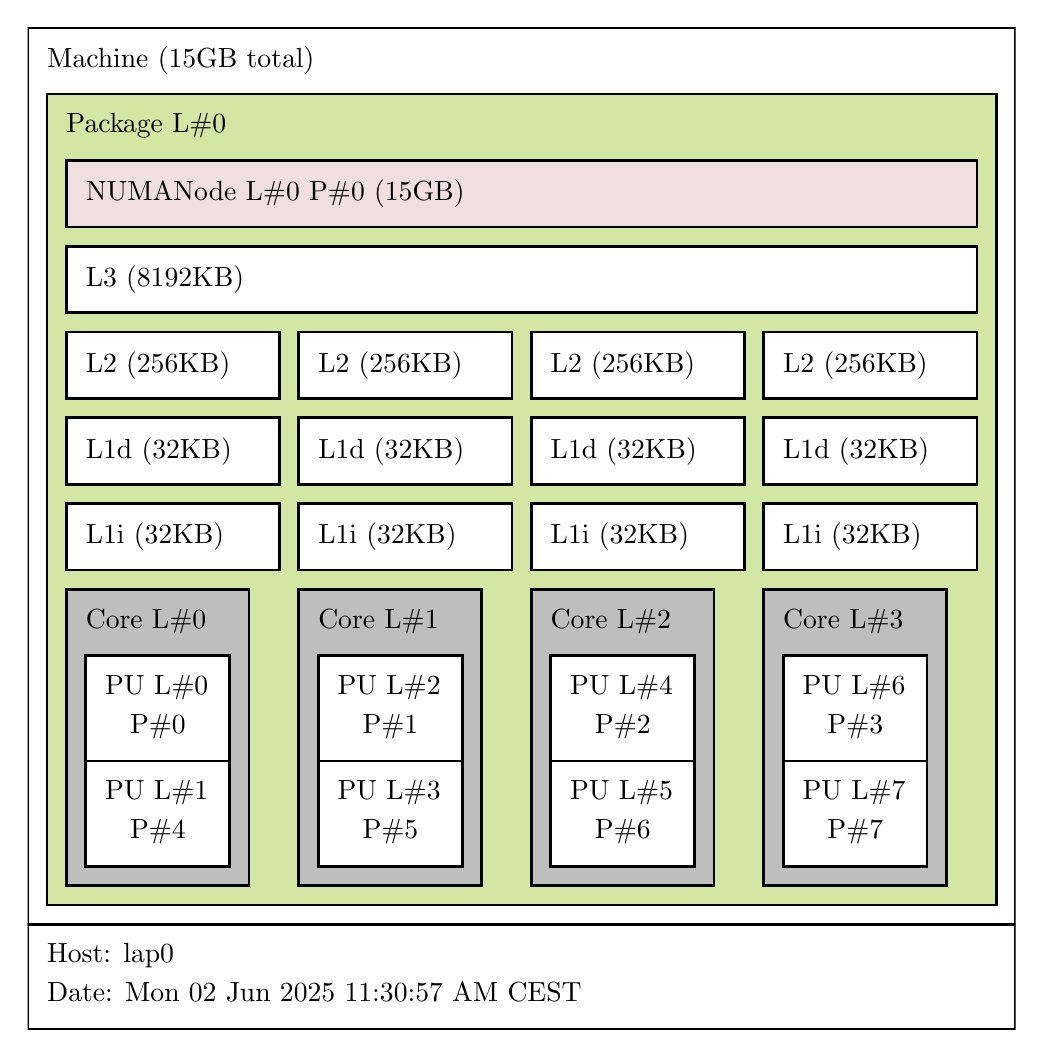
\begin{tikzpicture}[x=1pt,y=1pt,yscale=-1,hwloc-label/.style={fill=none,draw=none,text=black,align=left,anchor=north west,outer sep=0pt,inner sep=0pt,font=\fontsize{10}{14}\selectfont},hwloc-label-bold/.style={hwloc-label,font=\fontsize{10}{14}\selectfont\bfseries}]
	\clip (0,0) rectangle (357,362);
	\filldraw [fill=hwloc-color-255-255-255,draw=black,line width=1pt,solid] (0,0) rectangle ++(357,324);
	\node [hwloc-label,text=hwloc-color-0-0-0] at (7,7) {Machine (15GB total)};
	\filldraw [fill=hwloc-color-210-231-164,draw=black,line width=1pt,solid] (7,24) rectangle ++(343,293);
	\node [hwloc-label,text=hwloc-color-0-0-0] at (14,31) {Package L\#0};
	\filldraw [fill=hwloc-color-255-255-255,draw=black,line width=1pt,solid] (14,79) rectangle ++(329,24);
	\node [hwloc-label,text=hwloc-color-0-0-0] at (21,86) {L3 (8192KB)};
	\filldraw [fill=hwloc-color-255-255-255,draw=black,line width=1pt,solid] (14,110) rectangle ++(77,24);
	\node [hwloc-label,text=hwloc-color-0-0-0] at (21,117) {L2 (256KB)};
	\filldraw [fill=hwloc-color-255-255-255,draw=black,line width=1pt,solid] (14,141) rectangle ++(77,24);
	\node [hwloc-label,text=hwloc-color-0-0-0] at (21,148) {L1d (32KB)};
	\filldraw [fill=hwloc-color-255-255-255,draw=black,line width=1pt,solid] (14,172) rectangle ++(77,24);
	\node [hwloc-label,text=hwloc-color-0-0-0] at (21,179) {L1i (32KB)};
	\filldraw [fill=hwloc-color-190-190-190,draw=black,line width=1pt,solid] (14,203) rectangle ++(66,107);
	\node [hwloc-label,text=hwloc-color-0-0-0] at (21,210) {Core L\#0};
	\filldraw [fill=hwloc-color-255-255-255,draw=black,line width=1pt,solid] (21,227) rectangle ++(52,38);
	\node [hwloc-label,text=hwloc-color-0-0-0] at (28,234) {PU L\#0};
	\node [hwloc-label,text=hwloc-color-0-0-0] at (37,248) {P\#0};
	\filldraw [fill=hwloc-color-255-255-255,draw=black,line width=1pt,solid] (21,265) rectangle ++(52,38);
	\node [hwloc-label,text=hwloc-color-0-0-0] at (28,272) {PU L\#1};
	\node [hwloc-label,text=hwloc-color-0-0-0] at (37,286) {P\#4};
	\filldraw [fill=hwloc-color-255-255-255,draw=black,line width=1pt,solid] (98,110) rectangle ++(77,24);
	\node [hwloc-label,text=hwloc-color-0-0-0] at (105,117) {L2 (256KB)};
	\filldraw [fill=hwloc-color-255-255-255,draw=black,line width=1pt,solid] (98,141) rectangle ++(77,24);
	\node [hwloc-label,text=hwloc-color-0-0-0] at (105,148) {L1d (32KB)};
	\filldraw [fill=hwloc-color-255-255-255,draw=black,line width=1pt,solid] (98,172) rectangle ++(77,24);
	\node [hwloc-label,text=hwloc-color-0-0-0] at (105,179) {L1i (32KB)};
	\filldraw [fill=hwloc-color-190-190-190,draw=black,line width=1pt,solid] (98,203) rectangle ++(66,107);
	\node [hwloc-label,text=hwloc-color-0-0-0] at (105,210) {Core L\#1};
	\filldraw [fill=hwloc-color-255-255-255,draw=black,line width=1pt,solid] (105,227) rectangle ++(52,38);
	\node [hwloc-label,text=hwloc-color-0-0-0] at (112,234) {PU L\#2};
	\node [hwloc-label,text=hwloc-color-0-0-0] at (121,248) {P\#1};
	\filldraw [fill=hwloc-color-255-255-255,draw=black,line width=1pt,solid] (105,265) rectangle ++(52,38);
	\node [hwloc-label,text=hwloc-color-0-0-0] at (112,272) {PU L\#3};
	\node [hwloc-label,text=hwloc-color-0-0-0] at (121,286) {P\#5};
	\filldraw [fill=hwloc-color-255-255-255,draw=black,line width=1pt,solid] (182,110) rectangle ++(77,24);
	\node [hwloc-label,text=hwloc-color-0-0-0] at (189,117) {L2 (256KB)};
	\filldraw [fill=hwloc-color-255-255-255,draw=black,line width=1pt,solid] (182,141) rectangle ++(77,24);
	\node [hwloc-label,text=hwloc-color-0-0-0] at (189,148) {L1d (32KB)};
	\filldraw [fill=hwloc-color-255-255-255,draw=black,line width=1pt,solid] (182,172) rectangle ++(77,24);
	\node [hwloc-label,text=hwloc-color-0-0-0] at (189,179) {L1i (32KB)};
	\filldraw [fill=hwloc-color-190-190-190,draw=black,line width=1pt,solid] (182,203) rectangle ++(66,107);
	\node [hwloc-label,text=hwloc-color-0-0-0] at (189,210) {Core L\#2};
	\filldraw [fill=hwloc-color-255-255-255,draw=black,line width=1pt,solid] (189,227) rectangle ++(52,38);
	\node [hwloc-label,text=hwloc-color-0-0-0] at (196,234) {PU L\#4};
	\node [hwloc-label,text=hwloc-color-0-0-0] at (205,248) {P\#2};
	\filldraw [fill=hwloc-color-255-255-255,draw=black,line width=1pt,solid] (189,265) rectangle ++(52,38);
	\node [hwloc-label,text=hwloc-color-0-0-0] at (196,272) {PU L\#5};
	\node [hwloc-label,text=hwloc-color-0-0-0] at (205,286) {P\#6};
	\filldraw [fill=hwloc-color-255-255-255,draw=black,line width=1pt,solid] (266,110) rectangle ++(77,24);
	\node [hwloc-label,text=hwloc-color-0-0-0] at (273,117) {L2 (256KB)};
	\filldraw [fill=hwloc-color-255-255-255,draw=black,line width=1pt,solid] (266,141) rectangle ++(77,24);
	\node [hwloc-label,text=hwloc-color-0-0-0] at (273,148) {L1d (32KB)};
	\filldraw [fill=hwloc-color-255-255-255,draw=black,line width=1pt,solid] (266,172) rectangle ++(77,24);
	\node [hwloc-label,text=hwloc-color-0-0-0] at (273,179) {L1i (32KB)};
	\filldraw [fill=hwloc-color-190-190-190,draw=black,line width=1pt,solid] (266,203) rectangle ++(66,107);
	\node [hwloc-label,text=hwloc-color-0-0-0] at (273,210) {Core L\#3};
	\filldraw [fill=hwloc-color-255-255-255,draw=black,line width=1pt,solid] (273,227) rectangle ++(52,38);
	\node [hwloc-label,text=hwloc-color-0-0-0] at (280,234) {PU L\#6};
	\node [hwloc-label,text=hwloc-color-0-0-0] at (289,248) {P\#3};
	\filldraw [fill=hwloc-color-255-255-255,draw=black,line width=1pt,solid] (273,265) rectangle ++(52,38);
	\node [hwloc-label,text=hwloc-color-0-0-0] at (280,272) {PU L\#7};
	\node [hwloc-label,text=hwloc-color-0-0-0] at (289,286) {P\#7};
	\filldraw [fill=hwloc-color-239-223-222,draw=black,line width=1pt,solid] (14,48) rectangle ++(329,24);
	\node [hwloc-label,text=hwloc-color-0-0-0] at (21,55) {NUMANode L\#0 P\#0 (15GB)};
	\filldraw [fill=hwloc-color-255-255-255,draw=black,line width=1pt,solid] (0,324) rectangle ++(357,38);
	\node [hwloc-label,text=hwloc-color-0-0-0] at (7,331) {Host: lap0};
	\node [hwloc-label,text=hwloc-color-0-0-0] at (7,345) {Date: Mon 02 Jun 2025 11:30:57 AM CEST};
\end{tikzpicture}


}
  \caption[Testbed Memory Hierarchy]{The available testbed memory hierarchy. The four cores have to share the  8MB of available L3 cache.}
  \label{fig:topo}
\end{figure}

\section{Results}
\label{sec:res}
In this section, we will present and analyze the results. In figure~\ref{fig:cachemiss}, we can see the evolution of the cache miss rate, meaning the percentage of referenced memory lines that have to be loaded from main memory while running $q$ lookups on a tree with a total of $n$ nodes where $\text{Miss Rate (\%)}$ is computed as $\left( \frac{\text{Number of Cache Misses}}{\text{Total Memory Accesses}}. \right) \times 100$. Most notably, there are almost no cache misses for the VEB implementation, especially if we take the mandatory cache misses into account which are necessary in any case to initially bring the required lines into the cache. The pointer-based implementation consistently causes more cache misses. Specifically, after we increased the size of the tree to $n \ge 300000$, we can see an order of magnitude of more cache misses. 

\begin{figure}[H]
  \centering
  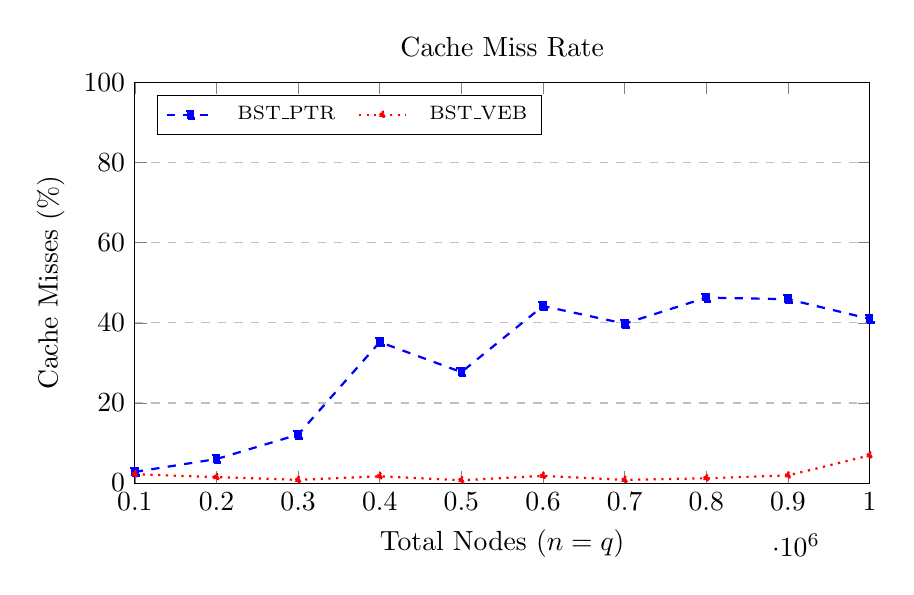
\begin{tikzpicture}
    \begin{axis}[
        title={Cache Miss Rate},
        xlabel={Total Nodes ($n=q$)},
        ylabel={Cache Misses (\%)},
        width =0.9\textwidth,
        height=0.55\textwidth,
        xmin=100000, xmax=1000000,
        ymin=0, ymax=100,
        ymajorgrids,
        grid style=dashed,
        legend columns=2,
        legend pos     = north west,
        legend style={font=\scriptsize, column sep=6pt},
    ]

    \addplot+[blue, thick, dashed, mark=square*, mark options={scale=.7,fill=blue}]
      coordinates {
        (100000,2.8) (200000,6.0) (300000,12.1) (400000,35.2)
        (500000,27.7) (600000,44.2) (700000,39.8) (800000,46.3)
        (900000,45.9) (1000000,41.0)
      };
    \addlegendentry{BST\_PTR}

    \addplot+[red, thick, dotted, mark=triangle*, mark options={scale=.7,fill=red}]
      coordinates {
        (100000,2.2) (200000,1.5) (300000,0.8) (400000,1.7)
        (500000,0.7) (600000,1.8) (700000,0.8) (800000,1.2)
        (900000,1.9) (1000000,6.9)
      };
    \addlegendentry{BST\_VEB}

    \end{axis}
  \end{tikzpicture}
  \caption{Cache miss rate (\%) as a function of total nodes and lookups ($n = q$) for the pointer-based (\texttt{BST\_PTR}) and VanEmde-Boas (\texttt{BST\_VEB}) implementations.}
  \label{fig:cachemiss}
\end{figure}


If we recall the available L3 cache memory in the testbed shown in figure~\ref{fig:topo} which is 8 MB, we can follow the plot seen in figure~\ref{fig:memory} and see that at $n=200000$, the memory required for the pointer-based implementation will amount to 4.4 MB which will likely fit into the cache, even though we have to consider other processes utilizing the cache. However, at  $n=300000$ we already require 6.5 MB of the total 8 MB which will likely cause contention on the cache which is expressed in the sudden increase in cache misses. Because of its much smaller memory footprint, the VEB implementation can basically fit the whole tree in L3 cache for the full series of input sizes up to $1.000.000$ (only 3.6 MB in VEB-layout) which results basically zero cache misses besides the mandatory ones. This means that up to this instance size, basically, no node has to be evicted upon a traversal because all nodes fit into the cache. 

\begin{figure}[H]
  \centering
  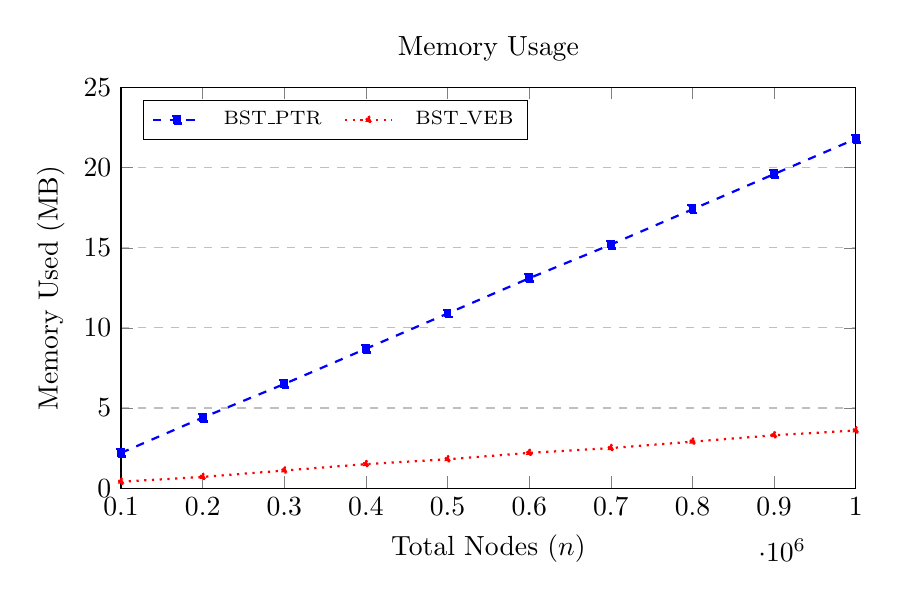
\begin{tikzpicture}
    \begin{axis}[
        title={Memory Usage},
        xlabel={Total Nodes ($n$)},
        ylabel={Memory Used (MB)},
        width =0.9\textwidth,
        height=0.55\textwidth,
        xmin=100000, xmax=1000000,
        ymin=0, ymax=25,
        ymajorgrids,
        grid style=dashed,
        legend columns=2,
        legend pos     = north west,
        legend style={font=\scriptsize, column sep=6pt},
    ]

    \addplot+[blue, thick, dashed, mark=square*, mark options={scale=.7,fill=blue}]
      coordinates {
        (100000,2.2) (200000,4.4) (300000,6.5) (400000,8.7)
        (500000,10.9) (600000,13.1) (700000,15.2) (800000,17.4)
        (900000,19.6) (1000000,21.8)
      };
    \addlegendentry{BST\_PTR}

    \addplot+[red, thick, dotted, mark=triangle*, mark options={scale=.7,fill=red}]
      coordinates {
        (100000,0.4) (200000,0.7) (300000,1.1) (400000,1.5)
        (500000,1.8) (600000,2.2) (700000,2.5) (800000,2.9)
        (900000,3.3) (1000000,3.6)
      };
    \addlegendentry{BST\_VEB}

    \end{axis}
  \end{tikzpicture}
  \caption{Memory usage in MB as a function of total nodes ($n$) for the pointer-based (\texttt{BST\_PTR}) and VanEmde-Boas (\texttt{BST\_VEB}) implementations.}
  \label{fig:memory}
\end{figure}

However, because of the slight increase in cache misses caused by the VEB towards the end of the plot, we will now discuss the results for bigger instances, as seen in figure~\ref{fig:cachemissbig} \& figure~\ref{fig:memorybig}. The VEB implementation consistently causes fewer cache misses, however, the percentage of misses of both implementations converges once we allocate more than $5.5 \times 10^6$ of nodes where the pointer implementation requires about 120 MB and the VEB-layout 20 MB. 
\begin{figure}[H]
  \centering
  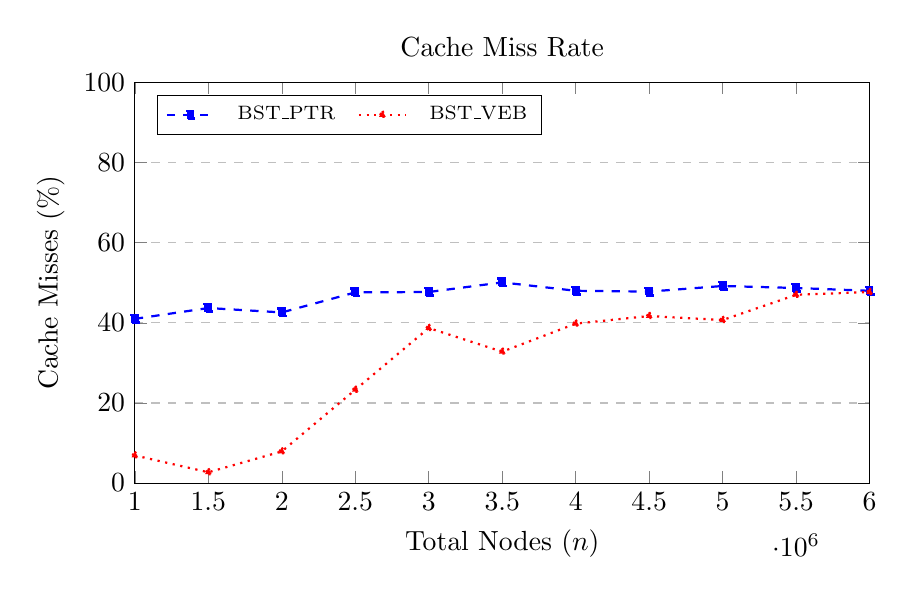
\begin{tikzpicture}
    \begin{axis}[
        title={Cache Miss Rate},
        xlabel={Total Nodes ($n$)},
        ylabel={Cache Misses (\%)},
        width=0.9\textwidth,
        height=0.55\textwidth,
        xmin=1000000, xmax=6000000,
        ymin=0, ymax=100,
        ymajorgrids,
        grid style=dashed,
        legend columns=2,
        legend pos=north west,
        legend style={font=\scriptsize, column sep=6pt},
    ]

    \addplot+[blue, thick, dashed, mark=square*, mark options={scale=.7,fill=blue}]
      coordinates {
        (1000000,41.0) (1500000,43.7) (2000000,42.6) (2500000,47.6)
        (3000000,47.7) (3500000,50.1) (4000000,48.0) (4500000,47.8)
        (5000000,49.2) (5500000,48.7) (6000000,48.0)
      };
    \addlegendentry{BST\_PTR}

    \addplot+[red, thick, dotted, mark=triangle*, mark options={scale=.7,fill=red}]
      coordinates {
        (1000000,6.9) (1500000,2.7) (2000000,7.9) (2500000,23.3)
        (3000000,38.7) (3500000,32.8) (4000000,39.8) (4500000,41.7)
        (5000000,40.7) (5500000,47.0) (6000000,47.7)
      };
    \addlegendentry{BST\_VEB}

    \end{axis}
  \end{tikzpicture}
  \caption{Cache miss rate (\%) as a function of total nodes and lookups ($q=1000000$) for the pointer-based (\texttt{BST\_PTR}) and VanEmde-Boas (\texttt{BST\_VEB}) implementations.}
  \label{fig:cachemissbig}
\end{figure}

\begin{figure}[H]
  \centering
  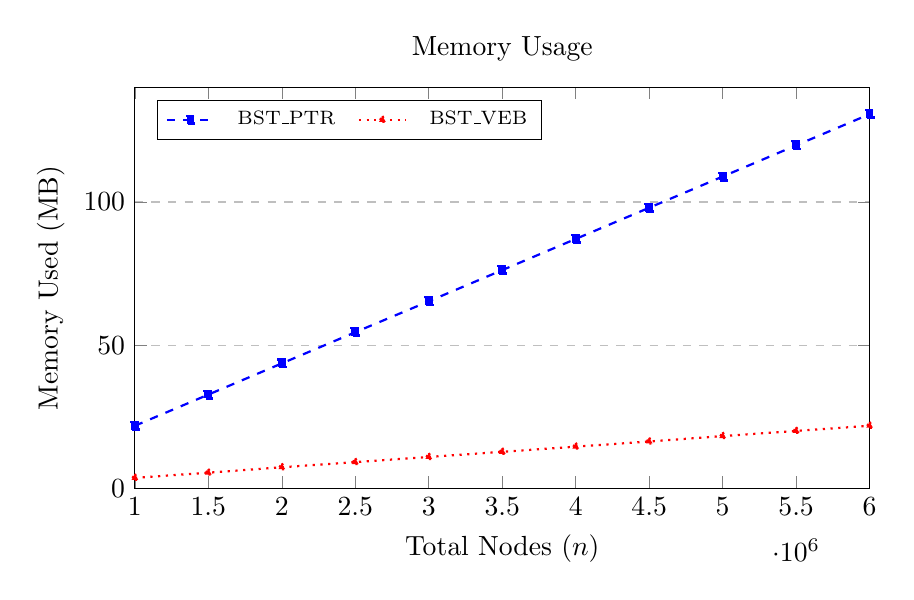
\begin{tikzpicture}
    \begin{axis}[
        title={Memory Usage},
        xlabel={Total Nodes ($n$)},
        ylabel={Memory Used (MB)},
        width=0.9\textwidth,
        height=0.55\textwidth,
        xmin=1000000, xmax=6000000,
        ymin=0, ymax=140,
        ymajorgrids,
        grid style=dashed,
        legend columns=2,
        legend pos=north west,
        legend style={font=\scriptsize, column sep=6pt},
    ]

    \addplot+[blue, thick, dashed, mark=square*, mark options={scale=.7,fill=blue}]
      coordinates {
        (1000000,21.8) (1500000,32.7) (2000000,43.6) (2500000,54.5)
        (3000000,65.3) (3500000,76.2) (4000000,87.1) (4500000,98.0)
        (5000000,108.9) (5500000,119.8) (6000000,130.7)
      };
    \addlegendentry{BST\_PTR}

    \addplot+[red, thick, dotted, mark=triangle*, mark options={scale=.7,fill=red}]
      coordinates {
        (1000000,3.6) (1500000,5.4) (2000000,7.3) (2500000,9.1)
        (3000000,10.9) (3500000,12.7) (4000000,14.5) (4500000,16.3)
        (5000000,18.2) (5500000,20.0) (6000000,21.8)
      };
    \addlegendentry{BST\_VEB}

    \end{axis}
  \end{tikzpicture}
  \caption{Memory usage in MB as a function of total nodes for the pointer-based (\texttt{BST\_PTR}) and VanEmde-Boas (\texttt{BST\_VEB}) implementations.}
  \label{fig:memorybig}
\end{figure}

Although the \texttt{miss} rate seems to be similar once we use bigger instances, a miss implies a reference to the L3 cache, meaning it was not found in L1 or L2. This becomes clear when we plot the needed references to L3 to complete $q = 1000000$ lookups seen in figure~\ref{fig:l3refs}. This means that even though the miss rate for the VEB layout may increase, more requested data fits into L1 and L2, resulting in fewer overall references to L3. When using the VEB layout, more nodes will fit into a cache line and additionally the nodes are mapped to memory such that a subtree root is followed up by its children which likely be in the same cache line or in a close one which will likely be prefetched. 
\begin{figure}[H]
  \centering
  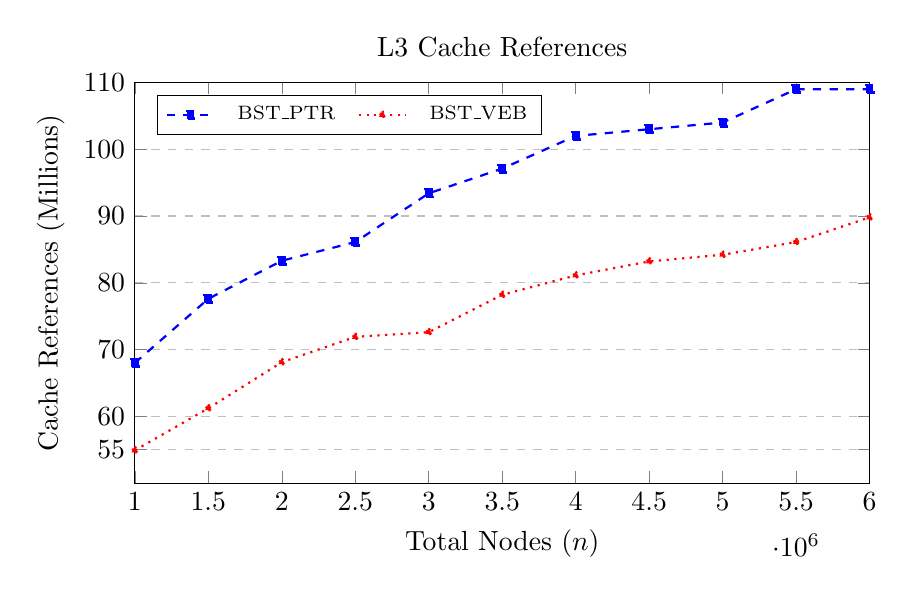
\begin{tikzpicture}
    \begin{axis}[
        title={L3 Cache References},
        xlabel={Total Nodes ($n$)},
        ylabel={Cache References (Millions)},
        width=0.9\textwidth,
        height=0.55\textwidth,
        xmin=1000000, xmax=6000000,
        ymin=5.0e7, ymax=1.1e8,
        ymajorgrids,
        grid style=dashed,
        legend columns=2,
        legend pos=north west,
        legend style={font=\scriptsize, column sep=6pt},
        scaled y ticks=false,
        ytick={5.5e7, 6e7, 7e7, 8e7, 9e7, 1e8, 1.1e8},
        yticklabels={55, 60, 70, 80, 90, 100, 110}
    ]

    \addplot+[blue, thick, dashed, mark=square*, mark options={scale=.7,fill=blue}]
      coordinates {
        (1000000,6.80e7) (1500000,7.76e7) (2000000,8.33e7) (2500000,8.61e7)
        (3000000,9.34e7) (3500000,9.71e7) (4000000,1.02e8) (4500000,1.03e8)
        (5000000,1.04e8) (5500000,1.09e8) (6000000,1.09e8)
      };
    \addlegendentry{BST\_PTR}

    \addplot+[red, thick, dotted, mark=triangle*, mark options={scale=.7,fill=red}]
      coordinates {
        (1000000,5.49e7) (1500000,6.12e7) (2000000,6.81e7) (2500000,7.19e7)
        (3000000,7.26e7) (3500000,7.82e7) (4000000,8.11e7) (4500000,8.32e7)
        (5000000,8.42e7) (5500000,8.61e7) (6000000,8.98e7)
      };
    \addlegendentry{BST\_VEB}

    \end{axis}
  \end{tikzpicture}
  \caption{L3 Cache references in millions as a function of total nodes for $q=1000000$ lookups for the pointer-based (\texttt{BST\_PTR}) and Van Emde Boas (\texttt{BST\_VEB}) implementations.}
  \label{fig:l3refs}
\end{figure}


\section{Conclusion}
In this assignment, we have introduced the theoretical concepts regarding the importance of cache-friendly data structure implementations. To this end, we studied how Van Emde-Boas (VEB) trees are implemented and laid out in physical memory and compared them to plain binary search trees (BST). We instrumented the codes such that we can measure their impact on the L3 cache using the \texttt{perf} framework. We collected metrics regarding the performance of the implementation, e.g. the total memory used, and found that the pointerless VEB trees have a smaller memory footprint compared to standard BST. In terms of cache misses, we found that we have to put the results into the context of the testbed we are running the benchmarks in: We were able to observe how the plain BST implementation uses up the scarce cache memory much faster and hence triggers an order of magnitude more cache misses once the L3 cache is full. While we already saw contention and eviction when allocating 300000 nodes in the pointer-base implementation, we were still able to keep the whole VEB tree in the cache for up to one million nodes where we observed the first signs of contention. We found that both implementations converge towards a 40\% miss rate if we increase the instance size to six million nodes. However, the VEB implementation required fewer references to the L3 cache overall, likely because it also improves locality on L1 and L2 caches. We were able to show how VEB trees improve cache friendliness and why they should be considered for relatively static cases where we do not have to insert and hence rebuild the layout frequently.    

\newpage
\section{Appendix}
\label{sec:app}
\subsection{\texttt{IBST.h}}
\begin{lstlisting}
#pragma once
#include <cstddef>

template<class Key>
class IBST {
public:
    virtual void insert(const Key& k)                = 0;
    virtual bool contains(const Key& k)        const = 0;
    virtual std::size_t size_bytes()           const = 0;
    virtual ~IBST() = default;
};
\end{lstlisting}
\captionof{lstlisting}[\texttt{IBST.h}]{Abstract interface class for our Binary Search Tree implementationin in \texttt{IBST.h}}
\label{lst:ibst}

\subsection{\texttt{BSTPtr.h}}
\begin{lstlisting}
#pragma once
#include "IBST.h"
#include <memory>
#include <utility>

template<class Key>
class BSTPtr : public IBST<Key> {
    struct Node {
        Key key;
        std::unique_ptr<Node> l, r;
        explicit Node(const Key& k) : key(k) {}
    };

    std::unique_ptr<Node> root_;
    std::size_t node_cnt_ = 0;

    void insertNode(std::unique_ptr<Node>& p, const Key& k) {
        if (!p) {
            p = std::make_unique<Node>(k);
            ++node_cnt_;                         
        } else if (k < p->key) {
            insertNode(p->l, k);
        } else if (k > p->key) {
            insertNode(p->r, k);
        }
    }

    static bool contains(const std::unique_ptr<Node>& p, const Key& k) {
        const Node* cur = p.get();
        while (cur) {
            if (k == cur->key) return true;
            cur = (k < cur->key) ? cur->l.get() : cur->r.get();
        }
        return false;
    }

public:
    void insert(const Key& k) override { insertNode(root_, k); }
    bool contains(const Key& k) const override { return contains(root_, k); }

    std::size_t size_bytes() const override { return node_cnt_ * sizeof(Node); }
};
\end{lstlisting}
\captionof{lstlisting}[\texttt{BSTPtr.h}]{Plain Binary Search Tree implementation in \texttt{BSTPtr.h}}
\label{lst:btspointer}

\subsection{\texttt{BSTVEB.h}}
\label{secsec:vb}
\begin{lstlisting}
#pragma once
#include "IBST.h"
#include <vector>
#include <algorithm>
#include <stdexcept>


namespace help {
template<class Key>
void build_veb(std::vector<Key>& out,
               const std::vector<Key>& sorted, std::size_t lo, std::size_t hi)
{
    if (lo >= hi) return;                       
    std::size_t mid = (lo + hi) / 2;            
    out.push_back(sorted[mid]);                 
    build_veb(out, sorted, lo, mid);            
    build_veb(out, sorted, mid + 1, hi);        
}
} 

template<class Key>
class BSTVEB : public IBST<Key> {
    std::vector<Key> a_;            
    bool              frozen_ = false;
    std::vector<Key>  inserts_;     


    void freeze() {
        if (frozen_) return;

        std::sort(inserts_.begin(), inserts_.end());
        inserts_.erase(std::unique(inserts_.begin(), inserts_.end()),
                       inserts_.end());

        a_.reserve(inserts_.size());
        help::build_veb(a_, inserts_, 0, inserts_.size());
        frozen_ = true;
    }

    bool containsRec(const Key& k,
                     std::size_t lo, std::size_t hi, std::size_t idx) const
    {
        if (lo >= hi) return false;            

        const Key& key = a_[idx];
        if (k == key) return true;

        std::size_t mid        = (lo + hi) / 2;
        std::size_t left_size  = mid - lo;    
        std::size_t left_idx   = idx + 1;   
        std::size_t right_idx  = idx + 1 + left_size;

        return (k < key)
             ? containsRec(k, lo, mid,           left_idx)
             : containsRec(k, mid + 1, hi,       right_idx);
    }

public:
    void insert(const Key& k) override {
        if (frozen_)
            throw std::logic_error("I am already frozen!");
        inserts_.push_back(k);
    }

    bool contains(const Key& k) const override {
        const_cast<BSTVEB*>(this)->freeze();   
        return containsRec(k, 0, a_.size(), 0);
    }

     std::size_t size_bytes() const override { return a_.size() * sizeof(Key); }
};

\end{lstlisting}
\captionof{lstlisting}[\texttt{BSTVEB.h}]{Van Emde-Boas Tree Implementation in \texttt{BSTVEB.h}}
\label{lst:btsvb}

\subsection{\texttt{benchmark.cpp}}
\label{secsec:bcpp}
\begin{lstlisting}
#include "IBST.h"
#include "BSTPtr.h"
#include "BSTVEB.h"
#include "PerfCounters.h"

#include <vector>
#include <random>
#include <iostream>
#include <iomanip>
#include <fstream>
#include "util/json.hpp"
#include <functional>
#include <chrono>

using json  = nlohmann::json;
using Clock = std::chrono::steady_clock;

struct Metrics {
    long long ns          = 0;
    long long ops         = 0;
    long long cache_refs  = 0;
    long long cache_miss  = 0;
};

template<class Key>
Metrics benchOnce(IBST<Key>& tree,
                  const std::vector<Key>& lookups,
                  const std::vector<Key>& inserts)
{
    for (const auto& k : inserts) tree.insert(k);

    PerfCounters pc;
    pc.start();

    auto start = Clock::now();
    for (const auto& k : lookups)
        (void)tree.contains(k);
    auto end   = Clock::now();

    pc.stop();

    Metrics m;
    m.ns         = std::chrono::duration_cast<std::chrono::nanoseconds>(end - start).count();
    m.ops        = lookups.size();
    m.cache_refs = pc.refs();
    m.cache_miss = pc.misses();
    return m;
}

using Factory = std::function<std::unique_ptr<IBST<int>>(void)>;
struct Variant { std::string name; Factory make; };

const std::vector<Variant> variants = {
    {"BST_PTR", [] { return std::make_unique<BSTPtr<int>>(); }},
    {"BST_VEB", [] { return std::make_unique<BSTVEB<int>>(); }},
};

void runExperiment(int n, int q, int T, bool csv,
                   const Factory& make, unsigned seed,
                   const std::string& impl)
{
    std::mt19937 rng(seed);
    std::uniform_int_distribution<int> dist(1, n * 10);

    std::vector<int> inserts(n);
    for (int& x : inserts) x = dist(rng);

    std::vector<int> lookups(q);
    for (int& x : lookups) x = dist(rng);

    long long  acc_ns   = 0;
    long long  acc_refs = 0, acc_miss = 0;
    std::size_t bytes_used = 0;

    for (int t = 0; t < T; ++t) {
        auto tree = make();
        Metrics m = benchOnce(*tree, lookups, inserts);
        acc_ns   += m.ns;
        acc_refs += m.cache_refs;
        acc_miss += m.cache_miss;
        if (t == 0) bytes_used = tree->size_bytes();  
    }

    double avg_ns      = double(acc_ns)   / T;
    double ns_per_op   = avg_ns / q;

    double avg_refs    = double(acc_refs) / T;
    double avg_miss    = double(acc_miss) / T;
    double miss_per_op = avg_miss / q;
    double miss_rate   = (avg_refs > 0) ? avg_miss / avg_refs : 0.0;  
    double avg_s       = avg_ns / 1e9;
    double bytes_mb    = bytes_used / 1024.0 / 1024.0;

    if (csv) {
        std::cout << impl << ','
                  << n << ',' << q << ','
                  << avg_ns << ','
                  << std::fixed << std::setprecision(2)
                  << avg_s << ','
                  << std::defaultfloat
                  << ns_per_op << ','
                  << avg_refs << ',' << avg_miss << ','
                  << miss_per_op << ','
                  << miss_rate << ','
                  << bytes_used  << '\n';
    } else {
        std::cout << std::fixed << std::setprecision(2)
                  << std::left
                  << std::setw(10) << impl
                  << std::setw(10) << n
                  << std::setw(10) << q
                  << std::setw(15) << avg_ns
                  << std::setw(10) << avg_s
                  << std::defaultfloat << std::setprecision(6)
                  << std::setw(15) << ns_per_op
                  << std::setw(15) << avg_refs
                  << std::setw(15) << avg_miss
                  << std::setw(12) << miss_per_op
                  << std::setw(10) << std::fixed << std::setprecision(3) << miss_rate
                  << std::setw(12) << std::fixed << std::setprecision(1) << bytes_mb
                  << '\n';
    }
}

int main(int argc, char* argv[])
{
    int         n    = 10000;
    int         q    = 10000;
    int         T    = 1;
    bool        csv  = false;
    unsigned    seed = 42;
    std::string impl = "ALL";

    if (argc >= 2) {
        std::ifstream in(argv[1]);
        if (!in) { std::cerr << "Cannot open " << argv[1] << '\n'; return 1; }
        json cfg; in >> cfg;
        if (cfg.contains("n"))    n    = cfg["n"];
        if (cfg.contains("q"))    q    = cfg["q"];
        if (cfg.contains("T"))    T    = cfg["T"];
        if (cfg.contains("csv"))  csv  = cfg["csv"];
        if (cfg.contains("seed")) seed = cfg["seed"];
        if (cfg.contains("impl")) impl = cfg["impl"];
    }

    if (argc == 3) impl = argv[2];

    if (!csv) {
        std::cout << std::left
                  << std::setw(10) << "impl"
                  << std::setw(10) << "n"
                  << std::setw(10) << "q"
                  << std::setw(15) << "total_ns"
                  << std::setw(10) << "total_s"
                  << std::setw(15) << "ns/search"
                  << std::setw(15) << "cache_refs"
                  << std::setw(15) << "cache_miss"
                  << std::setw(12) << "miss/search"
                  << std::setw(10) << "missRate"
                  << std::setw(12) << "bytes(MB)" << '\n'
                  << std::string(134, '-') << '\n';
    } else {
        std::cout << "impl,n,q,total_ns,total_s,ns_per_search,"
                     "cache_refs,cache_misses,misses_per_search,miss_rate,bytes\n";
    }

    for (const auto& v : variants) {
        if (impl != "ALL" && impl != v.name) continue;
        runExperiment(n, q, T, csv, v.make, seed, v.name);
    }
    return 0;
}

\end{lstlisting}
\captionof{lstlisting}[\texttt{BSTVEB.h}]{Benchmarking Driver in \texttt{benchmark.cpp}}
\label{lst:benchcpp}

\subsection{\texttt{PerfCounters.h}}
\label{secsec:perfsetup}
\begin{lstlisting}
#pragma once
#include <linux/perf_event.h>
#include <cstdint>         
#include <sys/syscall.h>    
#ifndef __NR_perf_event_open
#endif
#include <sys/ioctl.h>
#include <unistd.h>
#include <cstring>
#include <cerrno>
#include <stdexcept>
#include <array>

class PerfCounters {
    int fd_refs_{-1}, fd_misses_{-1};
    long long refs_{0}, misses_{0};

    static int openCounter(uint32_t type, uint64_t config)
    {
        perf_event_attr pea{};
        pea.type           = type;
        pea.size           = sizeof(perf_event_attr);
        pea.config         = config;
        pea.inherit        = 0;       
        pea.disabled       = 1;
        pea.exclude_kernel = 0;
        pea.exclude_hv     = 1;

        int fd = syscall(__NR_perf_event_open, &pea, 0, -1, -1, 0);
        if (fd == -1)
            throw std::runtime_error{"perf_event_open: " + std::string(strerror(errno))};
        return fd;
    }
public:
    PerfCounters()
    {
        fd_refs_   = openCounter(PERF_TYPE_HARDWARE, PERF_COUNT_HW_CACHE_REFERENCES);
        fd_misses_ = openCounter(PERF_TYPE_HARDWARE, PERF_COUNT_HW_CACHE_MISSES);
    }
    ~PerfCounters() { close(fd_refs_); close(fd_misses_); }

    inline void start() const { ioctl(fd_refs_, PERF_EVENT_IOC_RESET, 0); ioctl(fd_misses_, PERF_EVENT_IOC_RESET, 0);
                                ioctl(fd_refs_, PERF_EVENT_IOC_ENABLE, 0); ioctl(fd_misses_, PERF_EVENT_IOC_ENABLE, 0); }
    inline void stop()
{
    ioctl(fd_refs_,   PERF_EVENT_IOC_DISABLE, 0);
    ioctl(fd_misses_, PERF_EVENT_IOC_DISABLE, 0);

    if (read(fd_refs_, &refs_, sizeof(refs_))   != sizeof(refs_))
        throw std::runtime_error("failed to read cache-refs counter");
    if (read(fd_misses_, &misses_, sizeof(misses_)) != sizeof(misses_))
        throw std::runtime_error("failed to read cache-miss counter");
}
    long long refs()   const { return refs_;   }
    long long misses() const { return misses_; }
};

\end{lstlisting}
\captionof{lstlisting}[\texttt{PerfCounters.h}]{Instrumentation Setup for Perf in \texttt{PerfCounters.h}}
\label{lst:perfsetup}


\subsection{\texttt{small.json}}
\label{secsec:smalinstance}
\begin{lstlisting}
{
  "n"   : 100000,
  "q"   : 100000,
  "T"   : 5,
  "csv" : false,
  "seed": 123
}
\end{lstlisting}
\captionof{lstlisting}[\texttt{small.json}]{Example Instance in \texttt{small.json}}
\label{lst:exampleinstance}

\newpage
\printbibliography

\end{document}
